\chapter{FRF Experiment}
\label{chap:frf_experiment}

\chaptertoc{}

\begin{chapterabstract}
Put the abstract here.
\end{chapterabstract}


\section{Introduction}
\label{sec:frf_introduction}
Diffusion weighted magnetic resonance imaging (dMRI) has been widely used to probe the structure and organisation of brain tissue, with one particular area of focus being the estimation of the orientational distribution of neuronal fibres in a voxel. Many techniques have been developed for estimating this \ac{FOD}, a family of which are based on \ac{SD}.

While there are a variety of spherical deconvolution methods, the central principle is the same - the diffusion weighted signal as a function of the azimuthal ($\phi$) and elevation ($\theta$) angles is modelled as a spherical convolution of the \ac{FOD}, $F(\theta,\phi)$, with a kernel (called the \ac{FRF}), $R(\theta)$, the typical diffusion weighted signal from a single fibre population estimated a priori:
\begin{equation}
  S(\theta, \phi) = F(\theta, \phi) \otimes R(\theta) \,.
  \label{eq:spherical_conv}
\end{equation}

By modelling the signal in this way, a number of assumptions are made. Firstly, the contribution of the extra-axonal space to the signal is not explicitly modelled. This means that either the extra-axonal signal must be assumed to be identical to the intra-axonal signal (meaning that it can be included in the \ac{FRF}) or that the extra-axonal space has a negligible contribution to the total signal.

In fact, certain techniques using \ac{SD}, such \ac{AFD}, rely on the assumption that the extracellular signal is negligible at a high b-value (> 3000 \si{\second\per\milli\metre\squared}), though this has only been tested in simple numerical phantoms of straight parallel cylinders. 

Another assumption is that the \ac{FRF} is assumed to be the same for all fibres (or fibre populations) in the voxel, meaning that the overall signal is just this \ac{FRF} summed up across the orientations of all the fibres.
Additionally, this representation cannot properly account for non-straight fibres since an assumption is made that there is no exchange between fibres or, equivalently, between diffusion in different directions.
In essence, this means that the fibres are implicitly assumed to be perfectly straight and pointing a given direction since any deviation from straight (i.e. curved or undulating fibres) would add directions that are dependent on one another.

In practice, however, it is not possible to have a large number of straight fibres pointing in different directions within the same space and maintain a high fibre volume fraction other than in a few simple cases such as planar dispersed cylinders. Ex vivo studies using 3D electron microscopy of mouse corpus callosum have shown than axons are generally not straight, at least in part as a result of having to pack together around one another and other cells.

In this work we use \ac{ConFiG}, our recently developed white matter numerical phantom generator capable of generating realistic WM morphology, to investigate these whether these assumption hold in realistic axonal geometries. Firstly we investigate the contribution of the extracellular space to the total \ac{dMRI} signal, whether the extracellular signal is similar to intracellular signal and how much it contributes to the overall signal. Additional, we investigate how the realistic packing of fibres affects the diffusion within each fibre and whether the dMRI signal from each fibre is the same, as \ac{SD} assumes.

\section{Method}
\label{sec:frf_method}
% In order to test what impact the complex morphology introduced by packing fibres together has on the individual fibre response functions and how this varies from the straight fibre model used in SD a simulation experiment was performed in a set of numerical phantoms generated using ConFiG.
In order to test the assumptions in \ac{SD} techniques, experiments were performed in a range of numerical phantoms generated using ConFiG. In this section, we describe the phantoms that we generate and the \ac{dMRI} simulation experiments that were performed to probe these assumptions. 

\subsection{Phantom Generation}
\label{sec:frf_phantom_generation}
Two sets of phantoms were generated for this work, one set of phantoms containing a single bundle of fibres with varying amounts of orientation dispersion and one set of phantoms containing crossing bundles of fibres. The first set of phantoms are used in the first experiment to test whether the extracellular signal in a single bundle of fibres is similar to the intracellular signal and how much the extracelular signal from a single bundle of fibres contributes to the overall signal. Both the single bundle and crossing bundle phantoms were used in the second experiment to probe how the complex morphology introduced by packing fibres together impacts on the individual fibre response functions. 

% The fibres generated using \ac{ConFiG} are not simple straight cylinders since the fibres must bend and bulge to fit around one another.
Phantoms were generated for a single bundle of fibres with different amounts of \ac{OD}. A target \ac{OD} was generated for each phantom using orientations drawn from the Watson distribution \cite{Mardia2008} for $\kappa$ = 2, 6, 100.
%These values were chosen since $\kappa=6$ is a value which represents \ac{WM} in the corpus callosum well, as shown in \Cref{sec:config_result_dmri_sim}, while $\kappa=2$ represents an extreme of high dispersion and $\kappa=100$ represents an extreme of low dispersion.
A low $\kappa$ means high orientation dispersion, so phantoms with a lower $\kappa$ were expected to have more complex morphology since higher \ac{OD} means that they must grow around one another more to avoid intersections. A typical $\kappa$, estimated using \ac{NODDI} \cite{Zhang2012}, for the corpus callosum of a healthy \ac{HCP} \cite{Sotiropoulos2013a,VanEssen2012} subject is $\kappa \sim 6$, as demonstrated in \Cref{sec:config_results}.
Crossing bundle phantoms were generated by using starting and target points arrange into two or three crossing bundles and grown using \ac{ConFiG} to generate complex phantoms with interleaved fibres.

For testing individual fibre response functions, only the intracellular signal was needed since the ideal \ac{FRF} comes solely from the intracellular space. In this case, each fibre was rotated to be aligned with the $z-$axis and then extended with a reflected copy as in Lee et al. \cite{Lee2019a}.

% \todo[inline]{Here I want to quantify the microstructural complexity of the phantoms, primarily amount of undulation and amount of beading, to associate with variability in per-fibre FRF}

\subsection{dMRI simulation}
\label{sec:frf_dMRI_simulation}
Diffusion MRI signals were simulated from ConFiG phantoms using the Camino \ac{dMRI} simulator \cite{Cook2006,Hall2009} to perform the experiments described below. For all experiments a bulk diffusivity $D = \SI{2.0}{\micro\metre\squared\per\milli\second}$ was used in agreement with similar Monte Carlo experiments as in \Cref{sec:config_experiments} with standard Camino periodic boundaries \cite{Panagiotaki2010}.

\subsubsection{Extracellular contribution}
\label{sec:frf_method_extra}
To probe the contribution of the extracellular space on the overall signal, simulations were performed in \ac{ConFiG} phantoms using $10^5$ spins initialised uniformly space. All fibres in the \ac{ConFiG} phantoms were treated as impermeable, meaning that the intracellular and extracellular signals could be calculated independently by labelling which compartment each spin started in. As in \Cref{sec:config_experiments}, phantoms were extended with reflected copies.

Two different measurement schemes were used to assess the contribution of the extracellular space to the overall signal. Firstly, a radial scheme with 256 measurements equally space in the plane perpendicular to the main fibre direction with $b = 0, 1000, 2000, 3000, 5000, \SI{10000}{\second\per\milli\metre\squared}$ was used to assess how the extracellular signal decays in the radial direction where there should be the largest difference between intracellular and extracellular signals as in Raffelt et al. \cite{Raffelt2012}. Additionally, a scheme with the same b-values but directions equidistributed across the sphere was used to test how the signal varies in all directions.

\subsubsection{Per-fibre \ac{FRF}}

For each fibre 10,000 spins were initialised uniformly intra-axonal space and the simulations were performed using 5000 timesteps. A small set of test simulations were performed using 10$^5$ spins and 10$^4$ timesteps yielding negligibly different signals to these settings, so 10,000 and 5,000 were used for the main simulations. The measurement parameters were $\Delta = \SI{28}{\milli\second}$, $\delta = \SI{24}{\milli\second}$, $b = 0,1000,2000,3000,5000,\SI{10000}{\second\per\milli\metre\squared}$ and 256 gradient directions at each shell. This gives a diffusion time $d_t = \SI{20}{\milli\second}$ and $G = \SI{60}{\milli\tesla\per\metre}$ at $b = \SI{3000}{\second\per\milli\metre\squared}$, chosen to be a feasible gradient strength on a high-end clinical system.

To compare to the collection of straight fibres assumption implicit in the spherical deconvolution, a cylinder representing each fibre was generated using the endpoints of each fibre to give the direction and the mean radius of the fibre as the cylinder radius. The same measurement scheme was simulated in each cylinder in order to compare to the \ac{ConFiG} fibres. 

\subsection{Signal analysis}
\label{sec:frf_signal_analysis}

\subsubsection{Extracellular contribution}
\label{sec:frf_sig_proc_extra}

\subsubsection{Per-fibre \ac{FRF}}
\label{sec:frf_sig_proc_per_fibre}




\section{Results}
\label{sec:frf_results}

\subsection{Extracellular contribution}
\label{sec:frf_res_extracellular}

\begin{figure}
  \centering
  \begin{subfigure}[]{0.4\textwidth}
    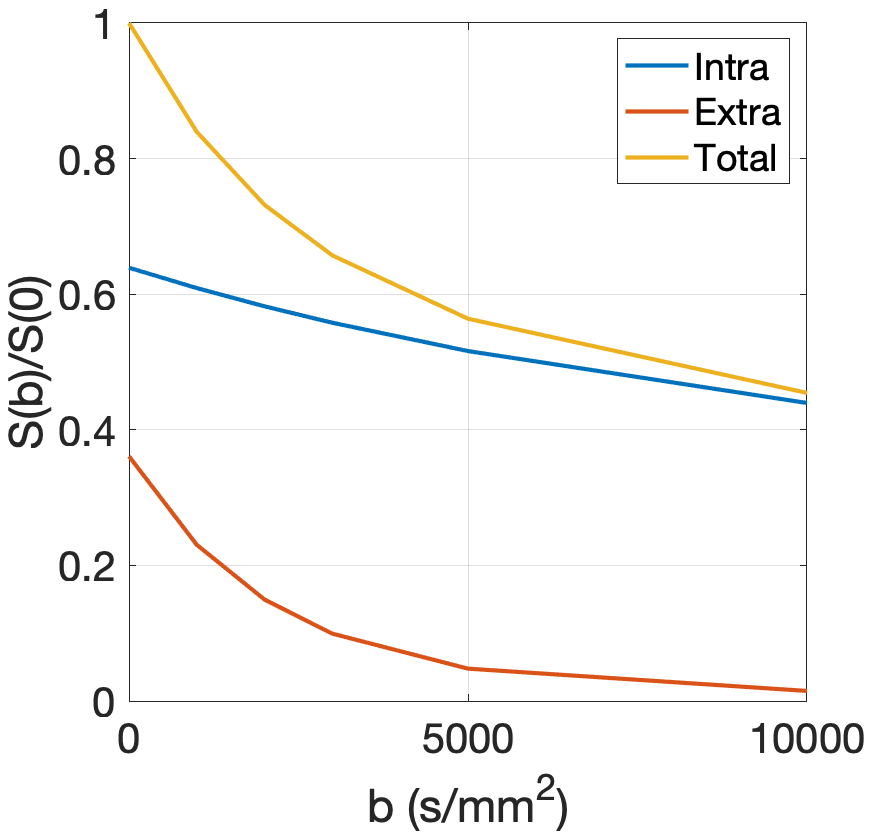
\includegraphics[width=\textwidth]{figures/frf_experiment/in_ex_tot_Kappa_2.png}
    \caption{}
  \end{subfigure}
  ~
  \begin{subfigure}[]{0.4\textwidth}
    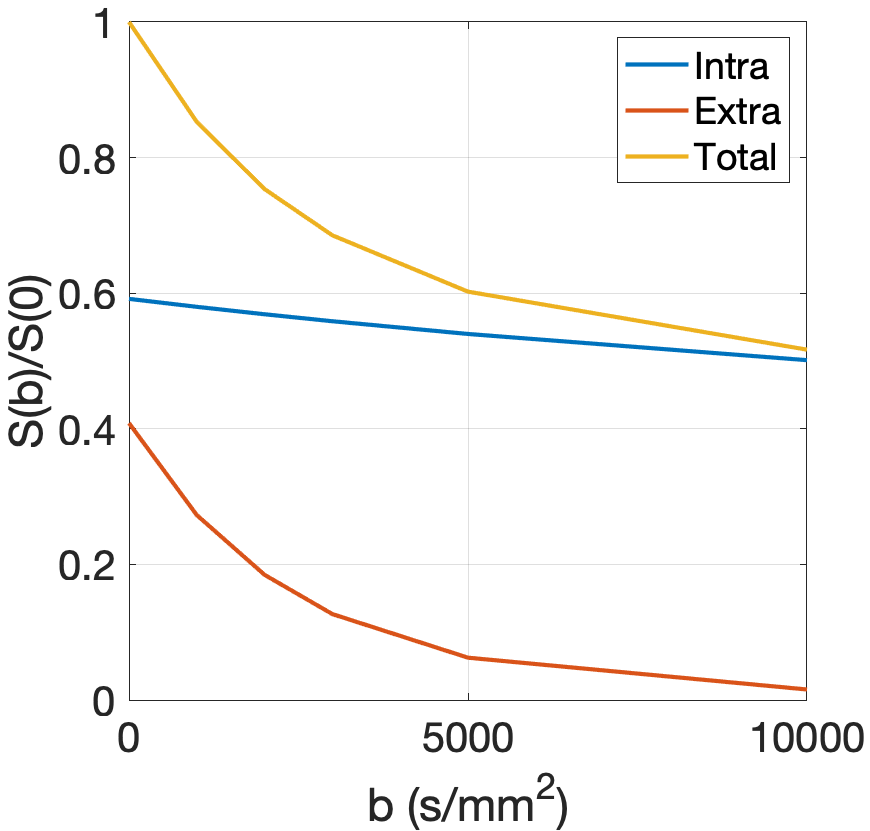
\includegraphics[width=\textwidth]{figures/frf_experiment/in_ex_tot_Kappa_6.png}
    \caption{}
  \end{subfigure}

  \begin{subfigure}[]{0.4\textwidth}
    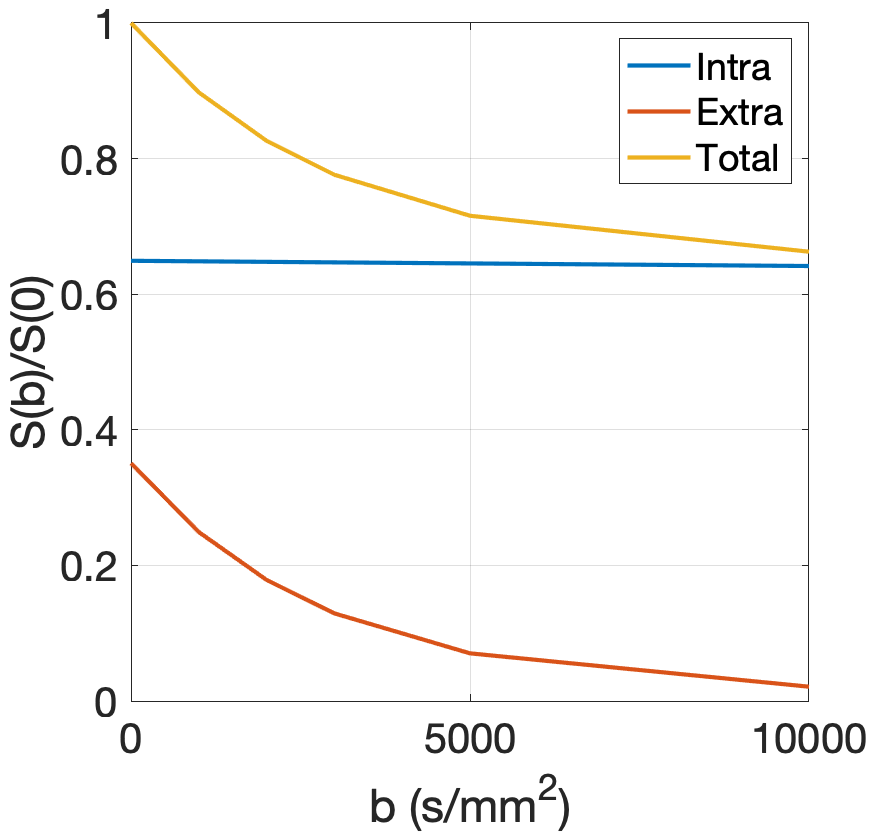
\includegraphics[width=\textwidth]{figures/frf_experiment/in_ex_tot_Kappa_100}
    \caption{}
  \end{subfigure}
  ~
  \begin{subfigure}[]{0.4\textwidth}
    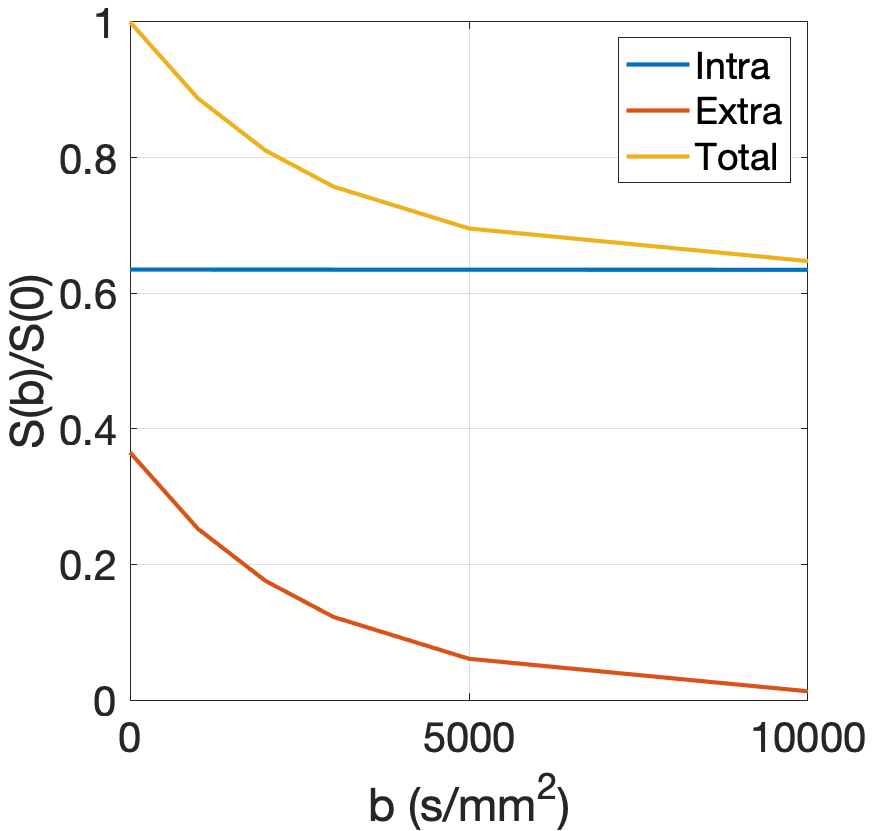
\includegraphics[width=\textwidth]{figures/frf_experiment/in_ex_tot_Gamma_Cylinders}
    \caption{}
  \end{subfigure}
  
  \caption[Intra, extra and overall signal as a function of b-value]{Intra, extra and overall radial signal as a function of b-value for (a) $\kappa=2$, (b) $\kappa=6$, (c) $\kappa=100$, (d) Cylinders.}
  \label{fig:frf_intra_ex_rad}
\end{figure}

\begin{figure}
  \centering
  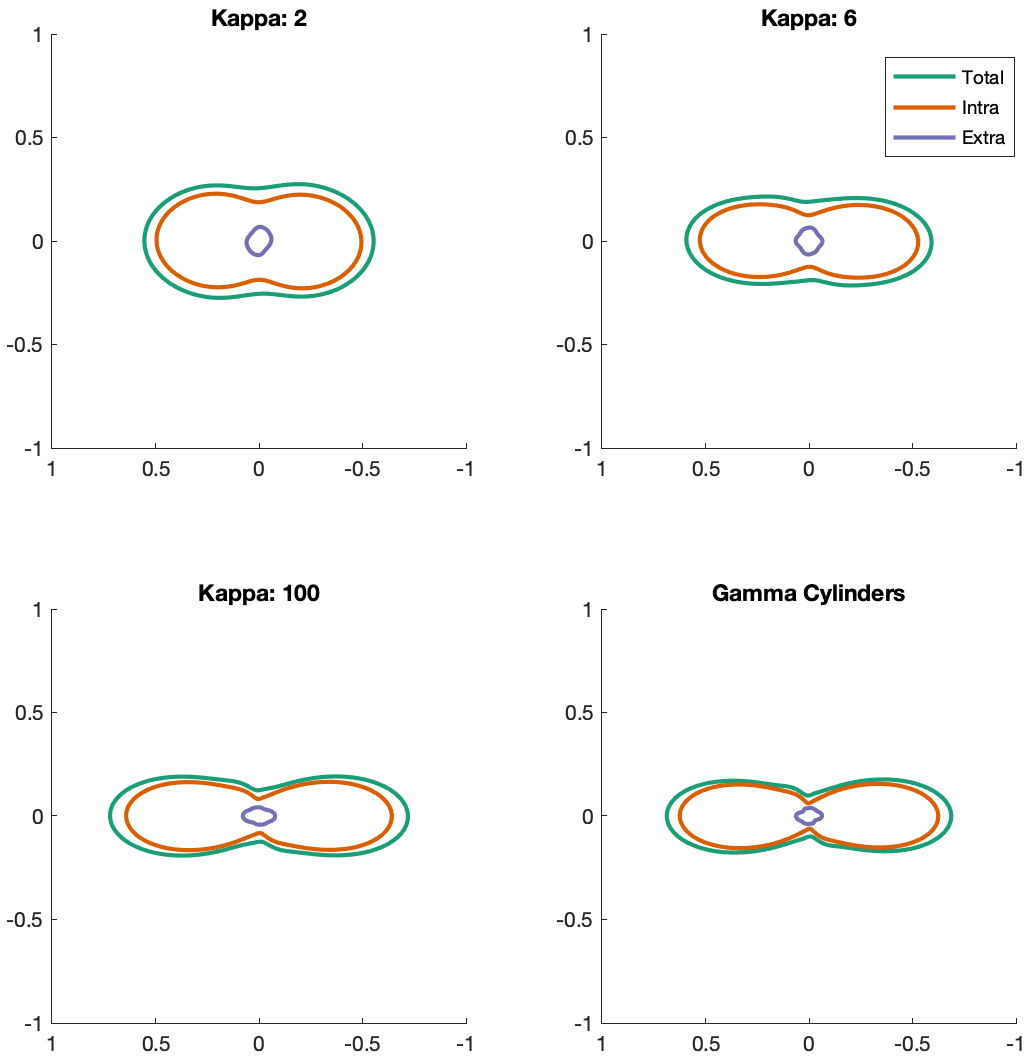
\includegraphics[width=0.85\textwidth]{figures/frf_experiment/sig_sh_b2000}
  \caption[Extracellular signal fraction as a function of b-value]{Total, intracellular and extracellular signal for $b = \SI{2000}{\second\per\milli\metre\squared}$ for a $\kappa = 2, 6$ and $100$ and straight parallel cylinders. }
  \label{fig:frf_extra_frac}
\end{figure}

\subsection{Per-fibre response function}
\label{sec:frf_res_per_fibre}


\begin{figure}
  \centering
  \begin{subfigure}[]{0.32\textwidth}
    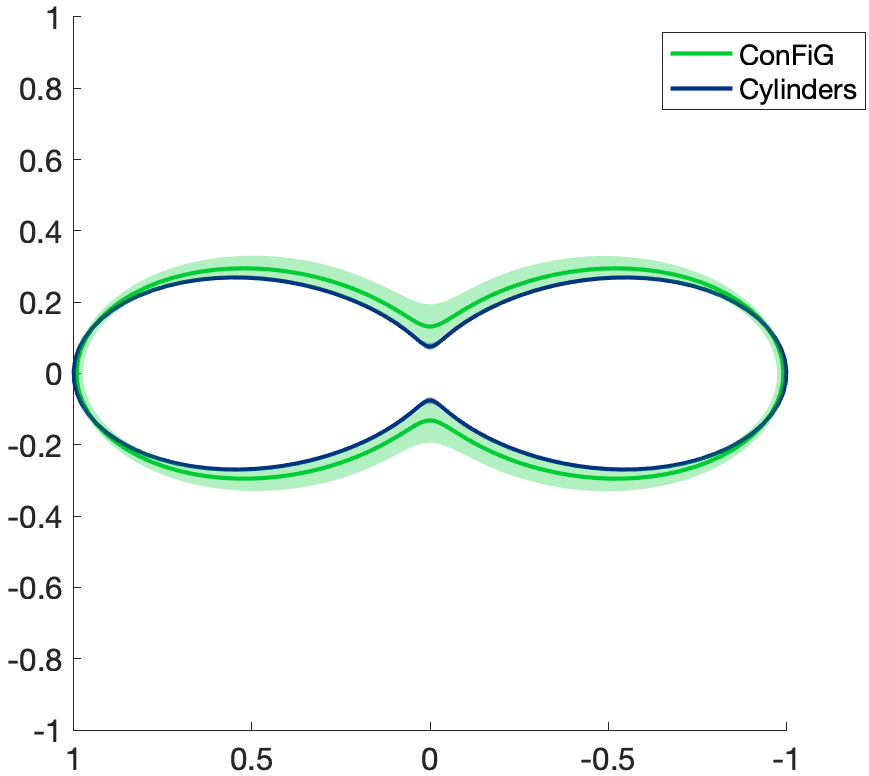
\includegraphics[width=\textwidth]{figures/frf_experiment/fibres_prctiles_kappa_2_b_2000.png}
    \caption{}
  \end{subfigure}
  ~
  \begin{subfigure}[]{0.32\textwidth}
    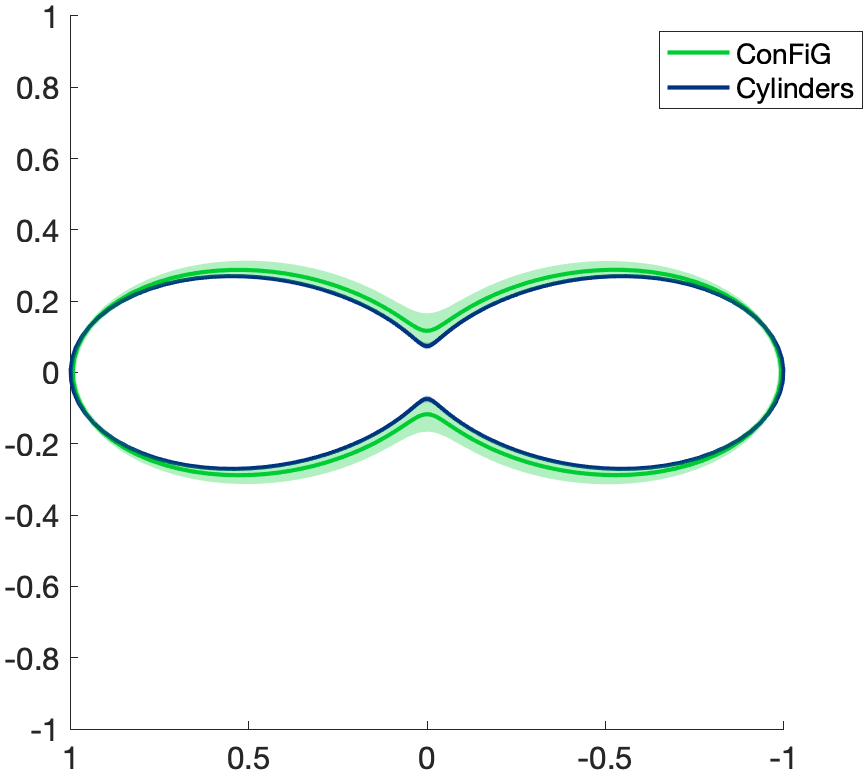
\includegraphics[width=\textwidth]{figures/frf_experiment/fibres_prctiles_kappa_6_b_2000.png}
    \caption{}
  \end{subfigure}
  ~
  \begin{subfigure}[]{0.32\textwidth}
    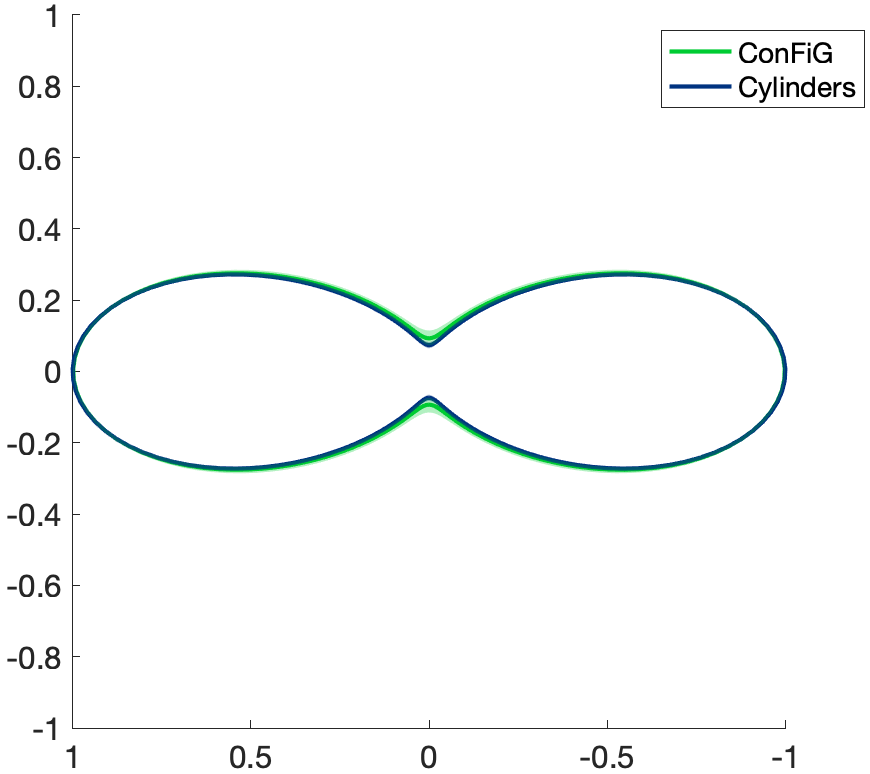
\includegraphics[width=\textwidth]{figures/frf_experiment/fibres_prctiles_kappa_100_b_2000.png}
    \caption{}
  \end{subfigure}

  \caption{Per-fibre FRF at $b = \SI{2000}{\second\per\milli\metre\squared}$ for (a) two crossing and (b) three crossing bundles of fibres. Solid line shows mean signal and shaded area shows 5th and 95th percentiles. }
  \label{fig:frf_prctiles_kappa_b2000}
\end{figure}

\begin{figure}
  \centering
  \begin{subfigure}[]{0.4\textwidth}
    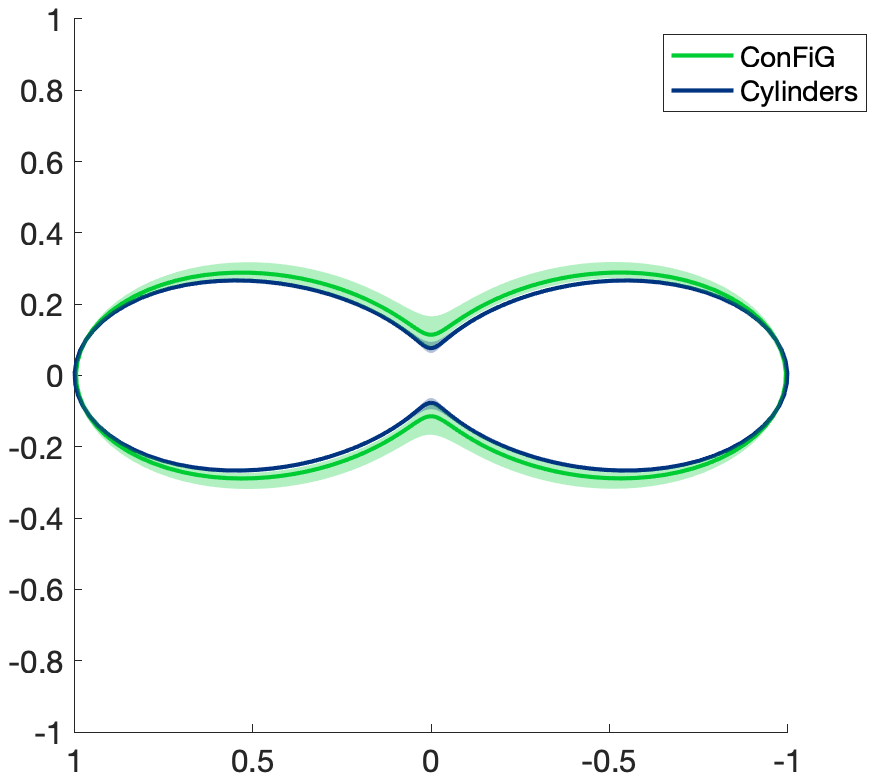
\includegraphics[width=\textwidth]{figures/frf_experiment/twoperp_prctiles_b_2000.png}
    \caption{}
  \end{subfigure}
  ~
  \begin{subfigure}[]{0.4\textwidth}
    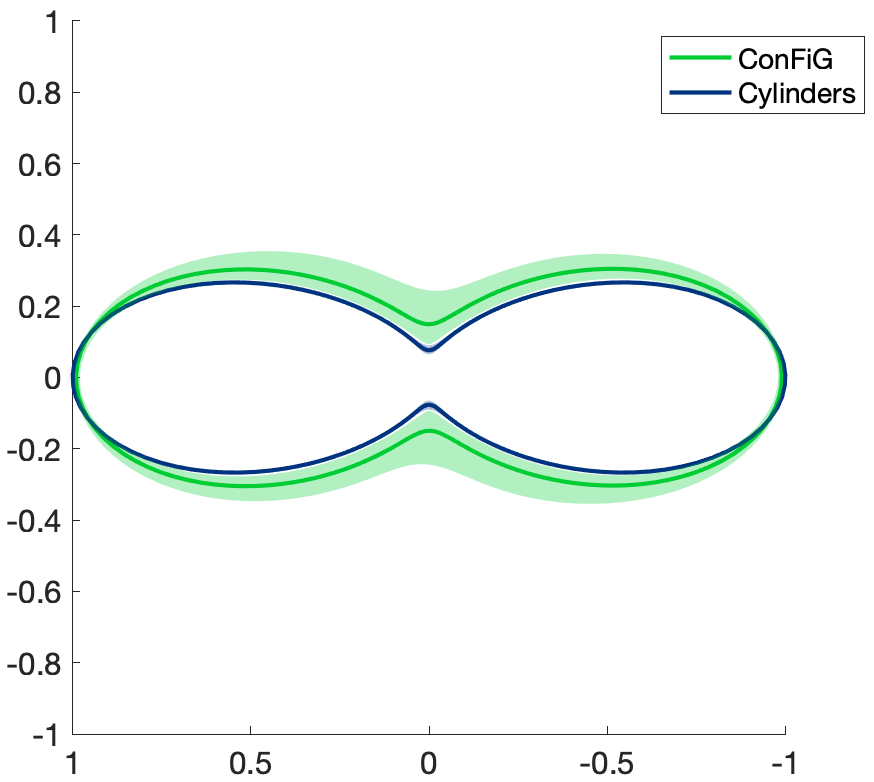
\includegraphics[width=\textwidth]{figures/frf_experiment/threeperp10deg_prctiles_b_2000.png}
    \caption{}
  \end{subfigure}

  \caption{Per-fibre FRF at $b = \SI{2000}{\second\per\milli\metre\squared}$ for $\kappa$ =(a)2, (b)6, (c)100. Solid line shows mean signal and shaded area shows 5th and 95th percentiles. }
  \label{fig:frf_prctiles_kappa_b2000}
\end{figure}

%%% Local Variables:
%%% mode: latex
%%% TeX-master: "../main"
%%% End:
